\documentclass[a4paper, 11pt]{article}
\usepackage{comment} % enables the use of multi-line comments (\ifx \fi) 
\usepackage{xparse}% http://ctan.org/pkg/xparse
\NewDocumentCommand{\Log}{o}{%
  \IfNoValueTF{#1}{}{{}^{#1}\!}\log}%
  
\usepackage{fullpage} % changes the margin
\usepackage{longtable}
\usepackage{graphicx}
\usepackage{fancyvrb,xcolor}
\usepackage{listings}
\usepackage{color, colortbl}
\usepackage[hyphenbreaks]{breakurl}
\usepackage[hyphens]{url}
\usepackage[margin=3cm]{geometry}
\usepackage{relsize}
\definecolor{dkgreen}{rgb}{0,0.6,0}
\definecolor{gray}{rgb}{0.5,0.5,0.5}
\definecolor{mauve}{rgb}{0.58,0,0.82}
\definecolor{LightCyan}{rgb}{0.88,1,1}
\usepackage{float}
\usepackage{caption}
\DeclareCaptionFont{white}{\color{white}}
\DeclareCaptionFormat{listing}{\colorbox{gray}{\parbox{\textwidth}{#1#2#3}}}
\captionsetup[lstlisting]{format=listing,labelfont=white,textfont=white}
\newcommand{\bigqm}[1][1]{\text{\larger[#1]{\textbf{?}}}}
\lstset{
  language=Java,
  aboveskip=3mm,
  belowskip=3mm,
  showstringspaces=false,
  columns=flexible,
  basicstyle={\small\ttfamily},
  numbers=none,
  numberstyle=\tiny\color{gray},
  keywordstyle=\color{blue},
  commentstyle=\color{dkgreen},
  stringstyle=\color{mauve},
  breaklines=true,
  breakatwhitespace=true,
  tabsize=3
}
\graphicspath{ {images/} }

\begin{document}
%Header-Make sure you update this information!!!!
\noindent
\large\textbf{Assignment 9} \hfill \textbf{Hussam Hallak} \\
\normalsize CS532, Web Science, Spring 2017\hfill CS Master's Student \\
Old Dominion University, Computer Science Dept \hfill Prof: Dr. Nelson 

\section*{Question 1:}
Choose a blog or a newsfeed (or something similar with an Atom
or RSS feed).  Every student should do a unique feed, so please
"claim" the feed on the class email list (first come, first served).
It should be on a topic or topics of which you are qualified to
provide classification training data.  Find something with at least
100 entries (or items if RSS).

Create between four and eight different categories for the entries
in the feed:

examples: 

work, class, family, news, deals

liberal, conservative, moderate, libertarian

sports, local, financial, national, international, entertainment

metal, electronic, ambient, folk, hip-hop, pop

Download and process the pages of the feed as per the week 12 
class slides.

Be sure to upload the raw data (Atom or RSS) to your github account.

Create a table with 100 rows, like:

\begin{lstlisting}[language=bash,label=Command:, breakatwhitespace=〈false), caption=Command:]

title									classification
-----									--------------
Ric Ocasek -								80s 
"Something To Grab 
For" (forgotten song)	

Weezer - "Pinkerton" 				alternative
(LP Review)

Schon \& Hammer - 							80s
"No More Lies" 
(forgotten song)

\end{lstlisting}

etc.  This is your "ground truth" (or "gold standard") data.


\subsection*{Answer:}

I claimed ``Programming Tutorials blog'' on blogspot:

http://tutorialsprogram.blogspot.com/

RSS Feed:

http://tutorialsprogram.blogspot.com/feeds/posts/default

The approach for grabbing 100 entries from the blog is divided into two steps:

1. Get the pages of the RSS feed. I modified the script, ``getpages.py'', I wrote for Assignment \#8 to use it to get all pages in the feed. I renamed the script ``getfeed.py''. it takes feed url as a command line argument. It gets all feed pages and saves the output to a file names ``pages.txt''.

\lstinputlisting[language=Python, breakatwhitespace=〈false), label=The content of getfeed.py, caption= The content of getfeed.py]{Q1/getfeed.py}

\begin{lstlisting}[language=bash, breakatwhitespace=〈false), label=Running getfeed.py, caption= Running getfeed.py]
root@ima-app:/var/www/Hussam/A9# python getfeed.py http://tutorialsprogram.blogspot.com/feeds/posts/default
root@ima-app:/var/www/Hussam/A9# ls
downloadrss.py  getfeed.py  pages.txt
root@ima-app:/var/www/Hussam/A9# cat pages.txt
http://tutorialsprogram.blogspot.com/feeds/posts/default
http://www.blogger.com/feeds/7802129033476755546/posts/default?start-index=26&max-results=25
https://www.blogger.com/feeds/7802129033476755546/posts/default?start-index=51&max-results=25
https://www.blogger.com/feeds/7802129033476755546/posts/default?start-index=76&max-results=25
https://www.blogger.com/feeds/7802129033476755546/posts/default?start-index=101&max-results=25
\end{lstlisting}

2. Get all entries in each feed page. I wrote a simple python script, ``downloadrss.py'', to do that using feedparser. It takes the feed url as a command line argument. It gets the title and the url for all entries and saves them to a file named ``rss.txt''

\lstinputlisting[language=Python, breakatwhitespace=〈false), label=The content of downloadrss.py, caption= The content of downloadrss.py]{Q1/downloadrss.py}

\begin{lstlisting}[language=bash, breakatwhitespace=〈false), label=Running downloadrss.py, caption= Running downloadrss.py]
root@ima-app:/var/www/Hussam/A9# python downloadrss.py http://tutorialsprogram.blogspot.com/feeds/posts/default
root@ima-app:/var/www/Hussam/A9# python downloadrss.py http://www.blogger.com/feeds/7802129033476755546/posts/default?start-index=26&max-results=25
root@ima-app:/var/www/Hussam/A9# python downloadrss.py https://www.blogger.com/feeds/7802129033476755546/posts/default?start-index=51&max-results=25
root@ima-app:/var/www/Hussam/A9# python downloadrss.py https://www.blogger.com/feeds/7802129033476755546/posts/default?start-index=76&max-results=25
root@ima-app:/var/www/Hussam/A9# python downloadrss.py https://www.blogger.com/feeds/7802129033476755546/posts/default?start-index=101&max-results=25
root@ima-app:/var/www/Hussam/A9# ls
downloadrss.py  getfeed.py  pages.txt  rss.txt
root@ima-app:/var/www/Hussam/A9# cat rss.txt | wc -l
120
root@ima-app:/var/www/Hussam/A9#
\end{lstlisting}

The file ``rss.txt'' is too big to include in this report, but here is a screen shot. The title and the url of each entry are saved on the same line separated by the ``pipe'' character.

\begin{figure}[H]
\centering
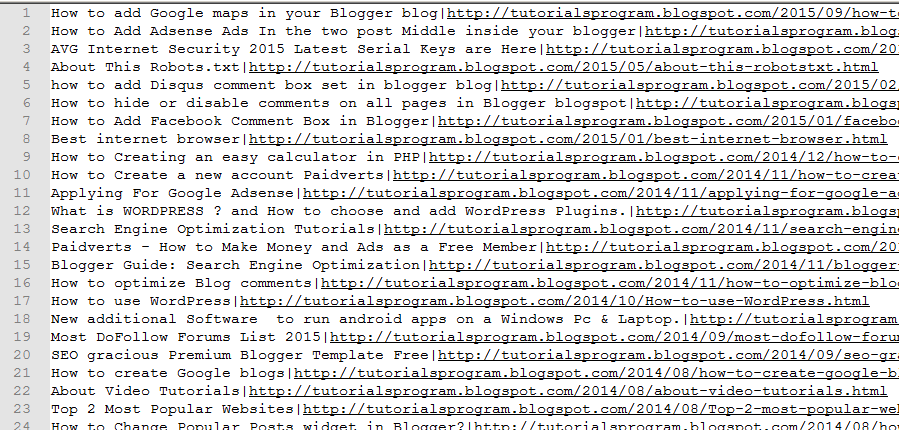
\includegraphics[scale=0.6]{rss.png}
\end{figure}

\textbf{Categories:}
I regretted claiming this blog because it is not rich nor is it organized to say the least. I am a full-time programmer, so I thought the best topic, for which I am qualified to provide classification training data, would be programming. I searched for programming tutorials blogs on blogspot in Google and randomly selected one of the results. I chose to have the following categories:

1. Tutorials

2. Articles

3. Downloads

4. Other

I finally created a simple python script, ``getrawdata.py'' to get the raw data. The script accepts the file ``pages.txt'' from the command line as input. It goes through each url in the input file and downloads the raw data, and saves it to files named 1.RawRSS, 2.RawRSS, 3.RawRSS, ...etc.

\lstinputlisting[language=Python, breakatwhitespace=〈false), label=The content of getrawdata.py, caption= The content of getrawdata.py]{Q1/getrawdata.py}

\begin{lstlisting}[language=bash, breakatwhitespace=〈false), label=Running getrawdata.py, caption= Running getrawdata.py]
root@ima-app:/var/www/Hussam/A9# python getrawdata.py pages.txt
root@ima-app:/var/www/Hussam/A9# ls
1.RawRSS  2.RawRSS  3.RawRSS  4.RawRSS  5.RawRSS  downloadrss.py  getfeed.py  getrawdata.py  pages.txt  rss.txt
root@ima-app:/var/www/Hussam/A9#
\end{lstlisting}

For the title-classification table, I will only use the first 100 entries per the question in the assignment. I saved the first 100 entries to a file and named it ``100rss.txt''. I manually categorized all 100 entries.
\begin{lstlisting}[language=bash]
root@ima-app:/var/www/Hussam/A9# head -n 100 rss.txt > 100rss.txt
root@ima-app:/var/www/Hussam/A9# ls
100rss.txt  1.RawRSS  2.RawRSS  3.RawRSS  4.RawRSS  5.RawRSS  downloadrss.py  getfeed.py  getrawdata.py  pages.txt  rss.txt
root@ima-app:/var/www/Hussam/A9#
\end{lstlisting}

For the table, I created a python script, ``maketable.py'', to generate LaTex code necessary to make the table. This is just to save typing time.

\lstinputlisting[language=Python, breakatwhitespace=〈false), label=The content of maketable.py, caption= The content of maketable.py]{Q1/maketable.py}

\begin{lstlisting}[language=bash, breakatwhitespace=〈false), label=Running maketable.py, caption= Running maketable.py]
root@ima-app:/var/www/Hussam/A9# python maketable.py 100rss.txt
root@ima-app:/var/www/Hussam/A9# ls
100rss.txt  1.RawRSS  2.RawRSS  3.RawRSS  4.RawRSS  5.RawRSS  downloadrss.py  getfeed.py  getrawdata.py  maketable.py  pages.txt  rss.txt  tex.table
root@ima-app:/var/www/Hussam/A9#
\end{lstlisting}


\begin{longtable}{ |p{12cm}|p{2cm}| }
\hline
Title
&
Classification \\
\hline
How to add Google maps in your Blogger blog
&
Tutorials \\
\hline
How to Add Adsense Ads In the two post Middle inside your blogger
&
Tutorials \\
\hline
AVG Internet Security 2015 Latest Serial Keys are Here
&
Downloads \\
\hline
About This Robots.txt
&
Articles \\
\hline
how to add Disqus comment box set in blogger blog
&
Tutorials \\
\hline
How to hide or disable comments on all pages in Blogger blogspot
&
Tutorials \\
\hline
How to Add Facebook Comment Box in Blogger
&
Tutorials \\
\hline
Best internet browser
&
Articles \\
\hline
How to Creating an easy calculator in PHP
&
Tutorials \\
\hline
How to Create a new account Paidverts
&
Articles \\
\hline
Applying For Google Adsense
&
Articles \\
\hline
What is WORDPRESS ? and How to choose and add WordPress Plugins.
&
Articles \\
\hline
Search Engine Optimization Tutorials
&
Tutorials \\
\hline
Paidverts - How to Make Money and Ads as a Free Member
&
Articles \\
\hline
Blogger Guide: Search Engine Optimization
&
Articles \\
\hline
How to optimize Blog comments
&
Tutorials \\
\hline
How to use WordPress
&
Tutorials \\
\hline
New additional Software  to run android apps on a Windows Pc \& Laptop.
&
Downloads \\
\hline
Most DoFollow Forums List 2015
&
Articles \\
\hline
SEO gracious Premium Blogger Template Free
&
Downloads \\
\hline
How to create Google blogs
&
Tutorials \\
\hline
About Video Tutorials
&
Other \\
\hline
Top 2 Most Popular Websites
&
Articles \\
\hline
How to Change Popular Posts widget in Blogger?
&
Tutorials \\
\hline
Mobogenie Aps Download PC and Android Phone
&
Downloads \\
\hline
Microworkers Forum Posting Jobs top secret explication
&
Articles \\
\hline
Start Earning From Micro-workers Jobs
&
Articles \\
\hline
Face-book Like box  For Blogger
&
Tutorials \\
\hline
Examples With Basic HTML  Tags
&
Others \\
\hline
Search Engine Optimization means that a Web site visitor through SEO- much increase
&
Articles \\
\hline
How to Earn Money Online in Site Building
&
Articles \\
\hline
Job as a Search Engine Optimization
&
Others \\
\hline
How To Remove Powered By Blogger Attribution From Blogger
&
Tutorials \\
\hline
About Author
&
Others \\
\hline
Free Blogger Templates For Blogspot
&
Downloads \\
\hline
How to SEO Optimize Archive Links in Blogger
&
Tutorials \\
\hline
How to Change The Background Color in Blogger?
&
Tutorials \\
\hline
How to add your blog Livefyre Comment System
&
Tutorials \\
\hline
Some of the Nokia  mobile  required code
&
Others \\
\hline
Hill Climb Racing for PC free Download Game (Windows 7
&
Downloads \\
\hline
How to add Twitter Flying bird Widget to Blog?
&
Tutorials \\
\hline
A Blog Widget
&
Others \\
\hline
About Internet
&
Articles \\
\hline
MOBILE PHONE APPLICATIONS
&
Articles \\
\hline
Introduction
&
Others \\
\hline
Introduction of HTML
&
Tutorials \\
\hline
About Programming Tutorials
&
Others \\
\hline
Background Properties
&
Tutorials \\
\hline
Background Properties\_\_CSS Background Color
&
Tutorials \\
\hline
Background Properties\_ CSS Text/Font Color
&
Tutorials \\
\hline
Types - External Style Sheet
&
Tutorials \\
\hline
Types - User Defined
&
Tutorials \\
\hline
Internal Styles - Identifiers
&
Tutorials \\
\hline
Internal Styles - Universal
&
Tutorials \\
\hline
CSS Style Types $>>$ Topic-01
&
Tutorials \\
\hline
Rule with CSS
&
Articles \\
\hline
HTML Anchor Tag
&
Tutorials \\
\hline
HTML $>>$ acronym/abbreviation
&
Articles \\
\hline
HTML Phrase Tags
&
Tutorials \\
\hline
Html $>>$ Canvas
&
Tutorials \\
\hline
Html  $>>$ Lists with HTML Bullets - (PART\_53)
&
Tutorials \\
\hline
Html $>>$  Subscript/Superscript - (PART\_52)
&
Tutorials \\
\hline
Html $>>$  Image tags - HTML form with submit button as image  - (PART\_51)
&
Tutorials \\
\hline
Html $>>$ Image tags- MAP/Image Mapping - (PART\_50)
&
Tutorials \\
\hline
HTML $>>$ DTD - Document Type Definition - (PART\_49)
&
Tutorials \\
\hline
Htm $>>$ HTML Tooltip  - (PART\_48)
&
Tutorials \\
\hline
Html $>>$ HTML Fieldset and Legend Tags  - (PART\_47)
&
Tutorials \\
\hline
Html $>>$ Frame tags >>Frames and Frameset Tag - (PART\_46)
&
Tutorials \\
\hline
Html $>>$ Meta Tag - (PART\_45)
&
Tutorials \\
\hline
Html $>>$ Media >>Embedding Video to HTML File - (PART\_44)
&
Tutorials \\
\hline
Html $>>$ Media >>Embedding Audio/Sound in background - (PART\_43)
&
Tutorials \\
\hline
Html  $>>$ CSS an Intro - (PART\_42)
&
Tutorials \\
\hline
Html  $>>$ Address Bar Icon in HTML page - (PART\_41)
&
Tutorials \\
\hline
Html $>>$ IFrame  tag - (PART\_40)
&
Tutorials \\
\hline
Html  $>>$ Auto refresh / Reload web page - (PART\_39)
&
Tutorials \\
\hline
Html  $>>$ Web Page Auto Redirection - (PART\_38)
&
Tutorials \\
\hline
Special/ASCII Characters in HTML - (PART\_37)
&
Tutorials \\
\hline
Forms $>>$  Html Label  - (PART\_36)
&
Tutorials \\
\hline
Forms $>>$ Html Password Field - (PART\_35)
&
Tutorials \\
\hline
Forms $>>$ Combo Box / Dropdown  - (PART\_34)
&
Tutorials \\
\hline
Forms $>>$ HTML TextArea Tag  - (PART\_33)
&
Tutorials \\
\hline
Forms $>>$ HTML Check Box Tag  - (PART\_32)
&
Tutorials \\
\hline
Forms $>>$ HTML Radio Button Tag  - (PART\_31)
&
Tutorials \\
\hline
Forms $>>$ HTML Button Tag - (PART\_30)
&
Tutorials \\
\hline
Forms $>>$ HTML Text Field Code - (PART\_29)
&
Tutorials \\
\hline
Forms>>  HTML Form Basic Types  - (PART\_28)
&
Tutorials \\
\hline
Using Tables $>>$ Table Row Span  - (PART\_27)
&
Tutorials \\
\hline
Using Tables $>>$ Table Col Span - (PART\_26)
&
Tutorials \\
\hline
Using Tables $>>$ Inner Tables - (PART\_25)
&
Tutorials \\
\hline
Using Tables    Table Alignment Code- (PART\_24)
&
Tutorials \\
\hline
Using Tables  $>>$ HTML Table Size - code  - (PART\_23)
&
Tutorials \\
\hline
Using Tables $>>$ Table Background Color and Image - (PART\_22)
&
Tutorials \\
\hline
Using Tables $>>$ HTML Table Border - (PART\_21)
&
Tutorials \\
\hline
Using Tables $>>$ Creating HTML Table - (PART\_20)
&
Tutorials \\
\hline
Special Effects $>>$ Special Effects - Blinking Text Tag- (PART\_19)
&
Tutorials \\
\hline
Special Effects $>>$ Special Effects - Marquee Tag- (PART\_18)
&
Tutorials \\
\hline
Special Effects $>>$ Special Effects - Marquee Tag -(PART\_17)
&
Tutorials \\
\hline
LINKS $>>$ Mail Link Code -(PART\_16)
&
Tutorials \\
\hline
LINKS $>>$ LINK Handling Code  -(PART\_15)
&
Tutorials \\
\hline
LINKS  $>>$   HTML LINKS Tag  -(PART\_14)
&
Tutorials \\
\hline
\end{longtable}



\subsection*{Included Files:}
1.RawRSS

\noindent
2.RawRSS

\noindent
3.RawRSS

\noindent
4.RawRSS

\noindent
5.RawRSS

\noindent
100rss.txt

\noindent
downloadrss.py

\noindent
getfeed.py

\noindent
getrawdata.py

\noindent
maketable.py

\noindent
pages.txt

\noindent
rss.png

\noindent
rss.txt

\noindent
tex.table

\section*{Question 2 \& 3:}
2. Train the Fisher classifier on the first 50 entries (the "training
set"), then use the classifier to guess the classification of the
next 50 entries (the "test set").

Create a table with 50 rows, like

\begin{lstlisting}[language=bash,label=Command:, breakatwhitespace=〈false), caption=Command:]

title								actual					predicted
-----								------					---------
Donnie Iris - 						80s							80s
"Ah! Leah!" 
(Forgotten Song)	

Black Sabbath - 					metal							metal
"Vol. 4" (LP Review)

Catherine Wheel - 				alternative					metal
"Ferment" (LP Review)

\end{lstlisting}

Assess the performance of your classifier in each of your categories
by computing precision, recall, and F-measure.  Use the "macro-averaged"
label based method, as per:

http://stats.stackexchange.com/questions/21551/how-to-compute-precision-recall-for-multiclass-multilabel-classification

For example, if you have 5 categories (e.g., 80s, metal,
alternative, electronic, cover), you will compute 
precision, recall, and F-measure for each category,
and then compute the average across the 5 categories.

3. Repeat question \#2, but use the first 90 entries to train your
classifier and the last 10 entries for testing.

\subsection*{Answer:}

I put the titles and the categories for the 100 entries in a text file named ``actual.txt''. Every entry and its classification are separated by the ``pipe'' character. and placed on one line in the file ``actual.txt''. The file is included in the folder ``Q2-3'' and here is a screen shot.

\begin{figure}[H]
\centering
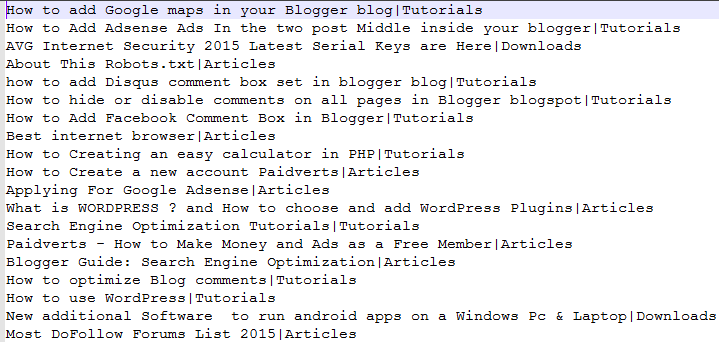
\includegraphics[scale=0.7]{actual.png}
\end{figure}

To perform the prediction, I wrote a small python program ``predict.py'' that takes the file ``actual.txt'' as input from the command line, and the program trains for the number of entries specified in the second command line argument, in this case 50 and then another run for 90, and predicts the classification for the number of entries specified in the third command line argument, 50 and then 10 entries in our case. The output is saved to a file in each run. These files are named ``predictedtable50\_50.txt'' and ``predictedtable90\_10''. The program imports the file ``docclass.py'' which is taken from ``PCI'' book and uses its functions ``train'' and ``classify'' to perform the training and the prediction.

\lstinputlisting[language=Python, breakatwhitespace=〈false), label=The content of predict.py, caption= The content of predict.py]{Q2-3/predict.py}

\begin{lstlisting}[language=bash, breakatwhitespace=〈false), label=Running predict.py: Training 50 Predicting 50, caption= Running predict.py: Training 50 Predicting 50]
root@ima-app:/var/www/Hussam/A9# python predict.py actual.txt 50 50
\end{lstlisting}

The file ``predictedtable50\_50.txt'' is then formatted to make the following table:

\begin{longtable}{ |p{10cm}|p{2cm}|p{2cm}| }
\hline
Title
&
Actual
&
Predicted \\
\hline
Types - External Style Sheet
&
Tutorials
&
Tutorials \\
\hline
Types - User Defined
&
Tutorials
&
Tutorials \\
\hline
Internal Styles - Identifiers
&
Tutorials
&
Tutorials \\
\hline
Internal Styles - Universal
&
Tutorials
&
Tutorials \\
\hline
CSS Style Types $>>$ Topic-01
&
Tutorials
&
Tutorials \\
\hline
\rowcolor{LightCyan}
Rule with CSS
&
Articles 
&
Tutorials\\
\hline
HTML Anchor Tag
&
Tutorials
&
Tutorials \\
\hline
\rowcolor{LightCyan}
HTML $>>$ acronym/abbreviation
&
Articles 
&
Tutorials \\
\hline
HTML Phrase Tags
&
Tutorials
&
Tutorials \\
\hline
Html $>>$ Canvas
&
Tutorials
&
Tutorials \\
\hline
Html  $>>$ Lists with HTML Bullets - (PART\_53)
&
Tutorials
&
Tutorials \\
\hline
Html $>>$  Subscript/Superscript - (PART\_52)
&
Tutorials
&
Tutorials \\
\hline
Html $>>$  Image tags - HTML form with submit button as image  - (PART\_51)
&
Tutorials
&
Tutorials \\
\hline
Html $>>$ Image tags- MAP/Image Mapping - (PART\_50)
&
Tutorials
&
Tutorials \\
\hline
HTML $>>$ DTD - Document Type Definition - (PART\_49)
&
Tutorials
&
Tutorials \\
\hline
Htm $>>$ HTML Tooltip  - (PART\_48)
&
Tutorials
&
Tutorials \\
\hline
Html $>>$ HTML Fieldset and Legend Tags  - (PART\_47)
&
Tutorials
&
Tutorials \\
\hline
Html $>>$ Frame tags >>Frames and Frameset Tag - (PART\_46)
&
Tutorials
&
Tutorials \\
\hline
Html $>>$ Meta Tag - (PART\_45)
&
Tutorials
&
Tutorials \\
\hline
Html $>>$ Media >>Embedding Video to HTML File - (PART\_44)
&
Tutorials
&
Tutorials \\
\hline
Html $>>$ Media >>Embedding Audio/Sound in background - (PART\_43)
&
Tutorials
&
Tutorials \\
\hline
Html  $>>$ CSS an Intro - (PART\_42)
&
Tutorials
&
Tutorials \\
\hline
Html  $>>$ Address Bar Icon in HTML page - (PART\_41)
&
Tutorials
&
Tutorials \\
\hline
Html $>>$ IFrame  tag - (PART\_40)
&
Tutorials
&
Tutorials \\
\hline
Html  $>>$ Auto refresh / Reload web page - (PART\_39)
&
Tutorials
&
Tutorials \\
\hline
Html  $>>$ Web Page Auto Redirection - (PART\_38)
&
Tutorials
&
Tutorials \\
\hline
Special/ASCII Characters in HTML - (PART\_37)
&
Tutorials
&
Tutorials \\
\hline
Forms $>>$  Html Label  - (PART\_36)
&
Tutorials
&
Tutorials \\
\hline
Forms $>>$ Html Password Field - (PART\_35)
&
Tutorials
&
Tutorials \\
\hline
Forms $>>$ Combo Box / Dropdown  - (PART\_34)
&
Tutorials
&
Tutorials \\
\hline
Forms $>>$ HTML TextArea Tag  - (PART\_33)
&
Tutorials
&
Tutorials \\
\hline
Forms $>>$ HTML Check Box Tag  - (PART\_32)
&
Tutorials
&
Tutorials \\
\hline
Forms $>>$ HTML Radio Button Tag  - (PART\_31)
&
Tutorials
&
Tutorials \\
\hline
Forms $>>$ HTML Button Tag - (PART\_30)
&
Tutorials
&
Tutorials \\
\hline
Forms $>>$ HTML Text Field Code - (PART\_29)
&
Tutorials
&
Tutorials \\
\hline
Forms>>  HTML Form Basic Types  - (PART\_28)
&
Tutorials
&
Tutorials \\
\hline
Using Tables $>>$ Table Row Span  - (PART\_27)
&
Tutorials
&
Tutorials \\
\hline
Using Tables $>>$ Table Col Span - (PART\_26)
&
Tutorials
&
Tutorials \\
\hline
Using Tables $>>$ Inner Tables - (PART\_25)
&
Tutorials
&
Tutorials \\
\hline
Using Tables    Table Alignment Code- (PART\_24)
&
Tutorials
&
Tutorials \\
\hline
Using Tables  $>>$ HTML Table Size - code  - (PART\_23)
&
Tutorials
&
Tutorials \\
\hline
Using Tables $>>$ Table Background Color and Image - (PART\_22)
&
Tutorials
&
Tutorials \\
\hline
Using Tables $>>$ HTML Table Border - (PART\_21)
&
Tutorials
&
Tutorials \\
\hline
Using Tables $>>$ Creating HTML Table - (PART\_20)
&
Tutorials
&
Tutorials \\
\hline
Special Effects $>>$ Special Effects - Blinking Text Tag- (PART\_19)
&
Tutorials
&
Tutorials \\
\hline
Special Effects $>>$ Special Effects - Marquee Tag- (PART\_18)
&
Tutorials
&
Tutorials \\
\hline
Special Effects $>>$ Special Effects - Marquee Tag -(PART\_17)
&
Tutorials
&
Tutorials \\
\hline
LINKS $>>$ Mail Link Code -(PART\_16)
&
Tutorials
&
Tutorials \\
\hline
LINKS $>>$ LINK Handling Code  -(PART\_15)
&
Tutorials
&
Tutorials \\
\hline
LINKS  $>>$   HTML LINKS Tag  -(PART\_14)
&
Tutorials
&
Tutorials \\
\hline
\end{longtable}

Now it's time to compute precision, recall, and F-measure for all four categories for both splits, 50/50 and 90/10. I manually calculated precision, recall, and F-measure from the values of True Positive, False Positive, False Negative for each category using the following formulas:
$$
Precision = \frac{TP}{TP+FP}
$$
$$
Recall = \frac{TP}{TP+FN}
$$
$$
F-measure = 2\times\frac{Precision \times Recall}{Precision + Recall}
$$

The unfortunate choice of the blog feed brought involved math into the calculations of the results. It is the frustrating problem of $\frac{0}{0}$. I am going with what math scientists call it, ``Indeterminate''.

\begin{longtable}{ |p{2cm}|p{0.5cm}|p{0.5cm}|p{0.5cm}|p{2.5cm}|p{2.5cm}|p{2.5cm}| }
\hline
Category
&
TP
&
FP
&
FN
&
Precision
&
Recall
&
F-Measure \\
\hline
Tutorials
&
48
&
2
&
0
&
0.96
&
1
&
0.98 \\
\hline
Articles
&
0
&
0
&
2
&
Indeterminate
&
0
&
Indeterminate \\
\hline
Downloads
&
0
&
0
&
0
&
Indeterminate
&
Indeterminate
&
Indeterminate \\
\hline
Other
&
0
&
0
&
0
&
Indeterminate
&
Indeterminate
&
Indeterminate \\
\hline
\end{longtable}

There is no way to compute the average across the categories because of the presence of indeterminate values.

\begin{lstlisting}[language=bash, breakatwhitespace=〈false), label=Running predict.py: Training 90 Predicting 10, caption= Running predict.py: Training 90 Predicting 10]
root@ima-app:/var/www/Hussam/A9# python predict.py actual.txt 90 10
\end{lstlisting}


The file ``predictedtable90\_10.txt'' is then formatted to make the following table:

\begin{longtable}{ |p{10cm}|p{2cm}|p{2cm}| }
\hline
Title
&
Actual
&
Predicted \\
\hline
Using Tables  $>>$ HTML Table Size - code  - (PART\_23)
&
Tutorials
&
Tutorials \\
\hline
Using Tables $>>$ Table Background Color and Image - (PART\_22)
&
Tutorials
&
Tutorials \\
\hline
Using Tables $>>$ HTML Table Border - (PART\_21)
&
Tutorials
&
Tutorials \\
\hline
Using Tables $>>$ Creating HTML Table - (PART\_20)
&
Tutorials
&
Tutorials \\
\hline
Special Effects $>>$ Special Effects - Blinking Text Tag- (PART\_19)
&
Tutorials
&
Tutorials \\
\hline
Special Effects $>>$ Special Effects - Marquee Tag- (PART\_18)
&
Tutorials
&
Tutorials \\
\hline
Special Effects $>>$ Special Effects - Marquee Tag -(PART\_17)
&
Tutorials
&
Tutorials \\
\hline
LINKS $>>$ Mail Link Code -(PART\_16)
&
Tutorials
&
Tutorials \\
\hline
LINKS $>>$ LINK Handling Code  -(PART\_15)
&
Tutorials
&
Tutorials \\
\hline
LINKS  $>>$   HTML LINKS Tag  -(PART\_14)
&
Tutorials
&
Tutorials \\
\hline
\end{longtable}

\begin{longtable}{ |p{2cm}|p{0.5cm}|p{0.5cm}|p{0.5cm}|p{2.5cm}|p{2.5cm}|p{2.5cm}| }
\hline
Category
&
TP
&
FP
&
FN
&
Precision
&
Recall
&
F-Measure \\
\hline
Tutorials
&
10
&
0
&
0
&
1
&
1
&
1 \\
\hline
Articles
&
0
&
0
&
0
&
Indeterminate
&
Indeterminate
&
Indeterminate \\
\hline
Downloads
&
0
&
0
&
0
&
Indeterminate
&
Indeterminate
&
Indeterminate \\
\hline
Other
&
0
&
0
&
0
&
Indeterminate
&
Indeterminate
&
Indeterminate \\
\hline
\end{longtable}

There is no way to compute the average across the categories because of the presence of indeterminate values.

\subsection*{Included Files:}

actual.txt

\noindent
predict.py

\noindent
predictedtable50\_50.txt

\noindent
predictedtable90\_10.txt

\noindent
docclass.py

\noindent
docclass.pyc

\noindent
hhallak.db

\end{document}
